\chapter{Реализация}

\begin{lstlisting}
#include <linux/fs.h>
#include <linux/init.h>
#include <linux/time.h>
#include <linux/slab.h>
#include <linux/kernel.h>
#include <linux/module.h>
#include <linux/version.h>

MODULE_LICENSE("GPL");
MODULE_AUTHOR("Faris Nabiev");

static int __init myfs_module_init(void);
static void __exit myfs_module_exit(void);

module_init(myfs_module_init);
module_exit(myfs_module_exit);

#define MYFS_MAGIC_NUMBER 0x13131313
#define SLABNAME "myfs_cache"

static int sco = 0;
// Размер элементов кэша
static int size = 7;
static int number = 31;
// Получение значения параметра командной строки
// если он передан
module_param(size, int, 0);
module_param(number, int, 0);

static void **line = NULL;

struct kmem_cache *cache = NULL;

static struct myfs_inode
{
     int i_mode;
     unsigned long i_ino;
} myfs_inode;

// Создание inode
static struct inode *myfs_make_inode(struct super_block *sb, int mode)
{
    // Размещение новой структуры inode
    struct inode *ret = new_inode(sb);

    if (ret)
    {
        inode_init_owner(ret, NULL, mode);

        // Заполнение значениями
        ret->i_size    = PAGE_SIZE;
        ret->i_atime   = ret->i_mtime = ret->i_ctime = current_time(ret);
        ret->i_private = &myfs_inode;
    }

    return ret;
}

// Деструктор суперблока, вызываемый перед уничтожением
// структуры super_block (при размонтировании ФС)
static void myfs_put_super(struct super_block * sb)
{
    printk(KERN_DEBUG "myfs: super block destroyed\n");
}

// Операции структуры суперблок
static struct super_operations const myfs_super_ops = {
    .put_super  = myfs_put_super,
    .statfs     = simple_statfs,
    .drop_inode = generic_delete_inode,
};

// Функция инициализации суперблока
// Выполняет построение корневого каталога ФС
static int myfs_fill_sb(struct super_block *sb, void *data, int silent)
{
    struct inode* root = NULL;

    // Заполняется структура super_block
    sb->s_blocksize      = PAGE_SIZE;
    sb->s_blocksize_bits = PAGE_SHIFT;
    sb->s_magic          = MYFS_MAGIC_NUMBER;
    sb->s_op             = &myfs_super_ops;

    // Создание inode каталога ФС (указывает на это S_IFDIR)
    root = myfs_make_inode(sb, S_IFDIR | 0755);
    if (!root)
    {
        printk (KERN_ERR "myfs: inode allocation failed\n");
        return -ENOMEM;
    }

    // Файловые и inode операции из libfs
    root->i_op  = &simple_dir_inode_operations;
    root->i_fop = &simple_dir_operations;

    // Создание структуры dentry для
    // представления корневого каталога в ядре
    sb->s_root = d_make_root(root);
    if (!sb->s_root)
    {
        printk(KERN_ERR "myfs: root creation failed\n");
        iput(root);
        return -ENOMEM;
    }

    return 0;
}

// Монтирование ФС
// возвращает структуру, описывающую корневой каталог ФС
static struct dentry* myfs_mount(struct file_system_type *type,
                                 int flags, char const *dev, void *data)
{
    // myfs_fill_sb будет вызвана по переданному указателю
    // из mount_bdev, чтобы проинициализировать суперблок
    struct dentry* const entry = mount_nodev(type, flags,
                                             data, myfs_fill_sb);

    if (IS_ERR(entry))
        printk(KERN_ERR "myfs: mounting failed\n");
    else
        printk(KERN_DEBUG "myfs: mounted\n");

    return entry;
}

// Описание создаваемой ФС
static struct file_system_type myfs_type = {
    // счетчик ссылок на модуль
    .owner   = THIS_MODULE,
    // название ФС
    .name    = "myfs",
    // указатель на функцию, вызываемую при монтировании ФС
    .mount   = myfs_mount,
    // указатель на функцию, вызываемую при размонтировании ФС
    .kill_sb = kill_litter_super,
};

// Конструктор, вызываемый при размещении каждого элемента
static void co(void* p)
{
    *(int*)p = (int)p;
    sco++;
}

// Инициализация модуля
static int __init myfs_module_init(void)
{
    int i;
    int ret;

    if (size < 0)
    {
        printk(KERN_ERR "myfs: invalid argument\n");
        return -EINVAL;
    }

    line = kmalloc(sizeof(void*) * number, GFP_KERNEL);

    if (line == NULL)
    {
        printk(KERN_ERR "myfs: kmalloc error\n" );
        kfree(line);
        return -ENOMEM;
    }

    for (i = 0; i < number; i++)
    {
        line[i] = NULL;
    }

    cache = kmem_cache_create(SLABNAME, size, 0, SLAB_HWCACHE_ALIGN, co);

    if (cache == NULL)
    {
        printk(KERN_ERR "myfs: kmem_cache_create error\n" );
        kmem_cache_destroy(cache);
        kfree(line);
        return -ENOMEM;
    }

    for (i = 0; i < number; i++)
    {
        if (NULL == (line[i] = kmem_cache_alloc(cache, GFP_KERNEL))) {
            printk(KERN_ERR "myfs: kmem_cache_alloc error\n");

            for (i = 0; i < number; i++)
            {
                kmem_cache_free(cache, line[i]);
            }

            kmem_cache_destroy(cache);
            kfree(line);
            return -ENOMEM;
        }
    }

    printk(KERN_INFO "myfs: allocate %d objects into slab: %s\n",
           number, SLABNAME);
    printk(KERN_INFO "myfs: object size %d bytes, full size %ld bytes\n",
           size, (long)size * number);
    printk(KERN_INFO "myfs: constructor called %d times\n", sco);

    ret = register_filesystem(&myfs_type);

    if (ret != 0)
    {
        printk(KERN_ERR "myfs: module cannot register filesystem\n");
        return ret;
    }

    printk(KERN_DEBUG "myfs: module loaded\n");
    return 0;
}

// Выгрузка модуля
static void __exit myfs_module_exit(void)
{
    int i;
    int ret;

    for (i = 0; i < number; i++)
        kmem_cache_free(cache, line[i]);

    kmem_cache_destroy(cache);
    kfree(line);

    ret = unregister_filesystem(&myfs_type);

    if (ret != 0)
        printk(KERN_ERR "myfs: module cannot unregister filesystem\n");

    printk(KERN_DEBUG "myfs: module unloaded\n");
}
\end{lstlisting}

\chapter{Результаты работы}

\begin{figure}[H]
    \centering
    \caption{Сборка}\label{img:scr1}
    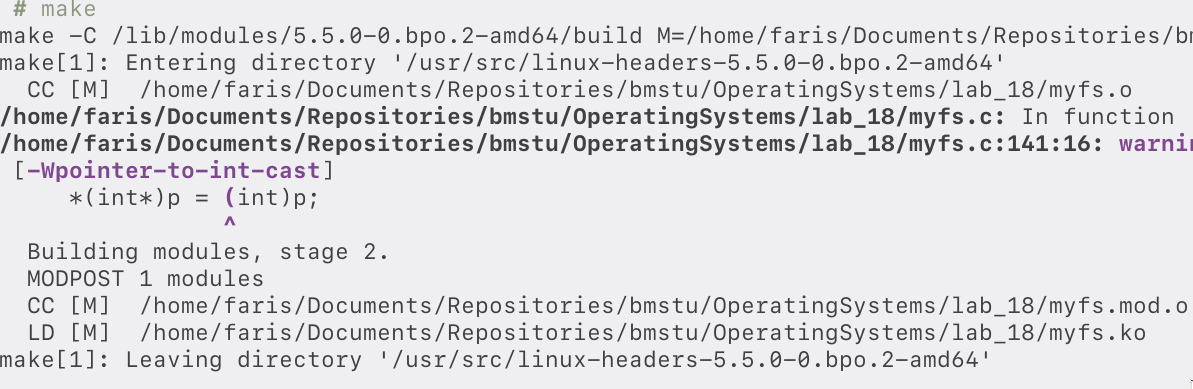
\includegraphics[scale=0.3]{images/scr1.png}
\end{figure}

\begin{figure}[H]
    \centering
    \caption{Загрузка модуля ядра и проверка списка загруженных модулей ядра}\label{img:scr2}
    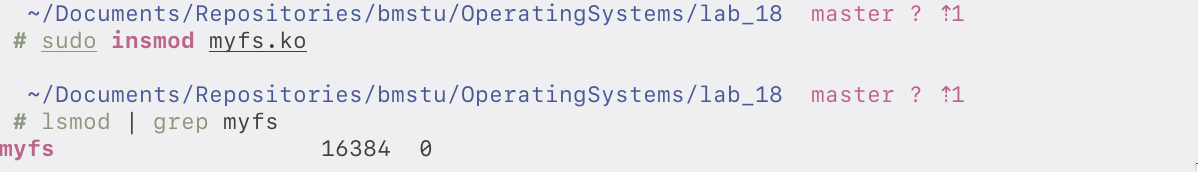
\includegraphics[scale=0.3]{images/scr2.png}
\end{figure}

\begin{figure}[H]
    \centering
    \caption{Вывод буфера сообщений ядра}\label{img:scr3}
    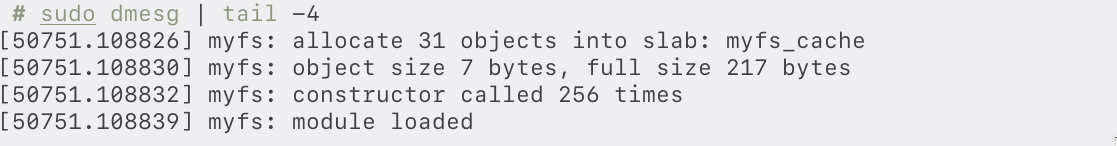
\includegraphics[scale=0.3]{images/scr3.png}
\end{figure}

\begin{figure}[H]
    \centering
    \caption{Состояние slab-кэша}\label{img:scr4}
    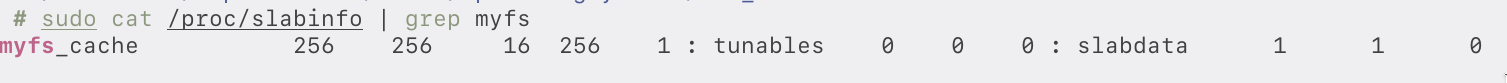
\includegraphics[scale=0.3]{images/scr4.png}
\end{figure}

\begin{figure}[H]
    \centering
    \caption{Создание образа диска, корня файловой системы; монтирование файловой системы}\label{img:scr5}
    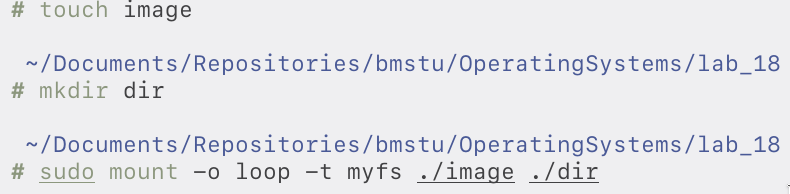
\includegraphics[scale=0.3]{images/scr5.png}
\end{figure}

\begin{figure}[H]
    \centering
    \caption{Вывод буфера сообщений ядра}\label{img:scr6}
    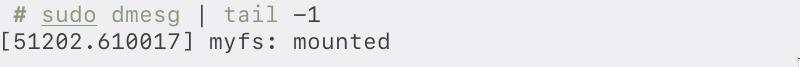
\includegraphics[scale=0.3]{images/scr6.png}
\end{figure}

\begin{figure}[H]
    \centering
    \caption{Вывод дерева каталогов}\label{img:scr7}
    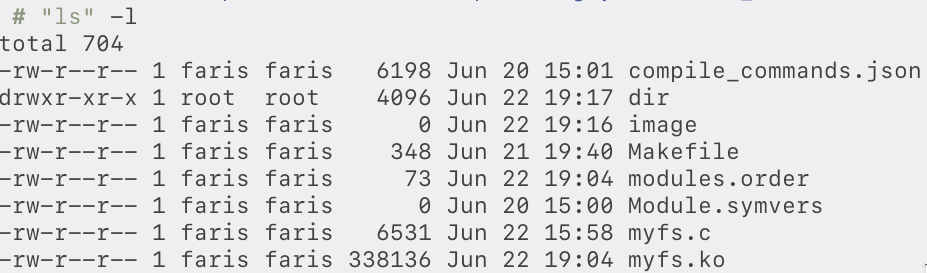
\includegraphics[scale=0.3]{images/scr7.png}
\end{figure}

\begin{figure}[H]
    \centering
    \caption{Размонтирование ФС и выгрузка модуля}\label{img:scr8}
    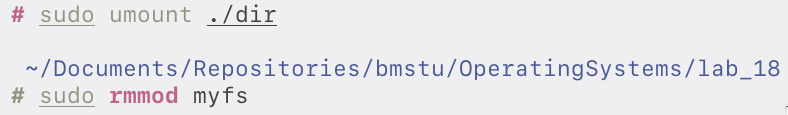
\includegraphics[scale=0.3]{images/scr8.png}
\end{figure}

\begin{figure}[H]
    \centering
    \caption{Вывод буфера сообщений ядра}\label{img:scr9}
    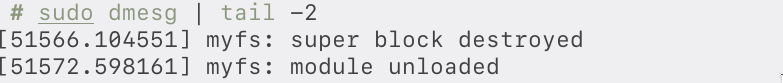
\includegraphics[scale=0.3]{images/scr9.png}
\end{figure}

\begin{figure}[H]
    \centering
    \caption{Загрузка модуля с заданным размером и количеством элементов кэша}\label{img:scr10}
    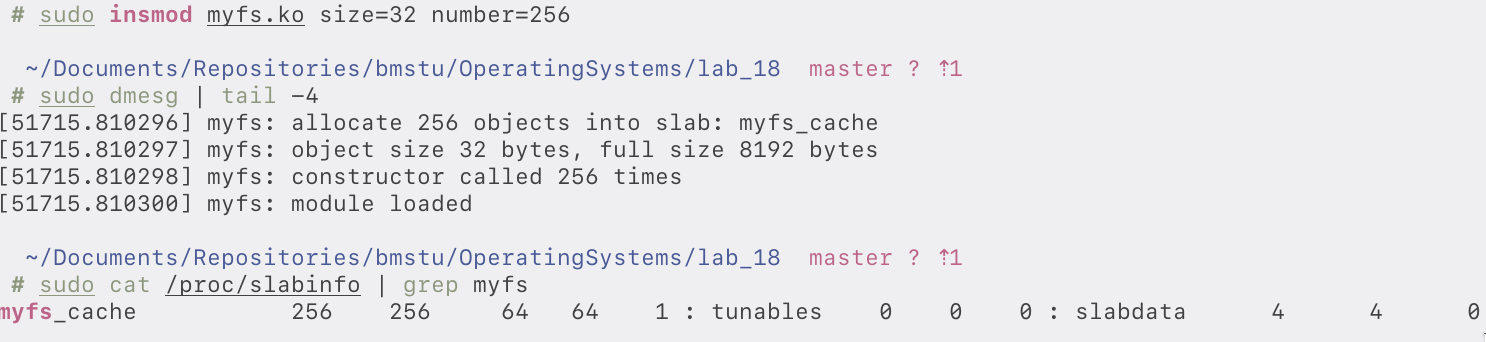
\includegraphics[scale=0.3]{images/scr10.png}
\end{figure}
